\NewDocumentCommand{\drawunit}{mm}
{
    \lPoint{O}{#1}
    \lShift{A}{O}{\fpeval{#2+90}:0.125}
    \lShift{B'}{A}{\fpeval{#2+180}:0.3}
    \lShift{C'}{A}{\fpeval{#2+0}  :0.3}
    \lShift{B}{B'}{\fpeval{#2-90}:0.25}
    \lShift{C}{C'}{\fpeval{#2-90}:0.25}
    \draw[rotate=#2,very thin,fill=blue!20!white] (A) rectangle (B);
    \draw[rotate=#2,very thin,fill=red!20!white ] (A) rectangle (C);
    \lRatio{Btext}{A}{B}{0.5}
    \lRatio{Ctext}{A}{C}{0.5}
    \node[rotate=#2] at (Btext) {\footnotesize S};
    \node[rotate=#2] at (Ctext) {\footnotesize N};
}

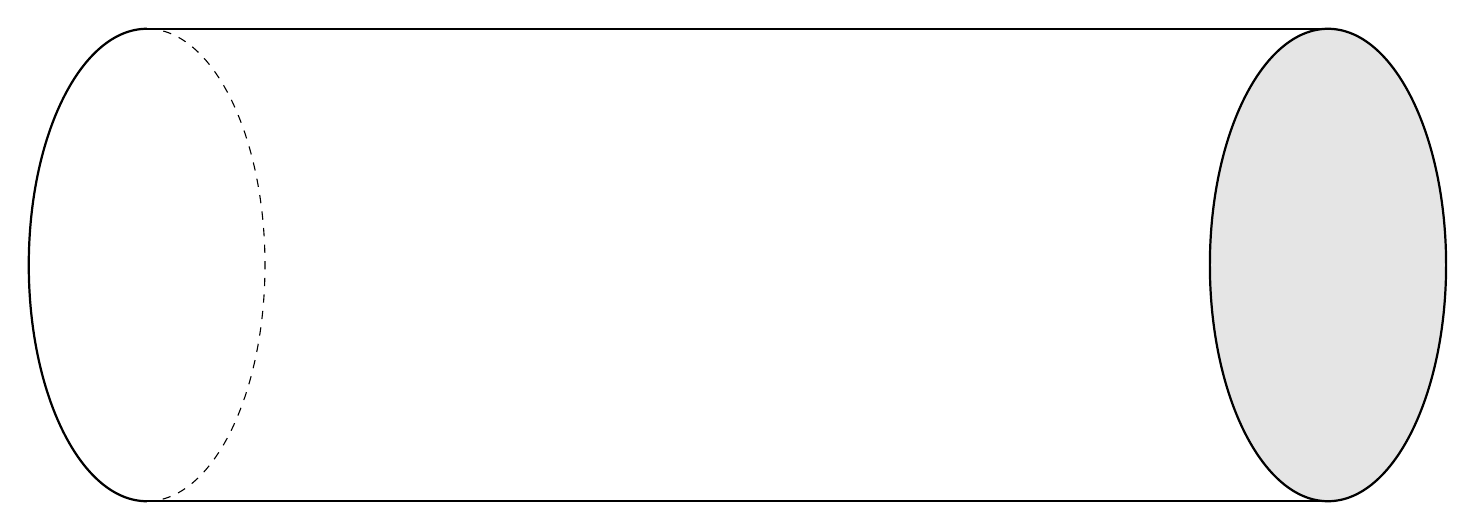
\begin{tikzpicture}[scale=1.5]
    \drawunit{-5.0,-1.2}{211}
    \drawunit{-5.0,-0.4}{179}
    \drawunit{-5.0,0.4}{252}
    \drawunit{-5.0,1.2}{15}
    \drawunit{-4.0,-1.2}{79}
    \drawunit{-4.0,-0.4}{348}
    \drawunit{-4.0,0.4}{117}
    \drawunit{-4.0,1.2}{65}
    \drawunit{-3.0,-1.2}{151}
    \drawunit{-3.0,-0.4}{40}
    \drawunit{-3.0,0.4}{246}
    \drawunit{-3.0,1.2}{353}
    \drawunit{-2.0,-1.2}{188}
    \drawunit{-2.0,-0.4}{145}
    \drawunit{-2.0,0.4}{302}
    \drawunit{-2.0,1.2}{347}
    \drawunit{-1.0,-1.2}{180}
    \drawunit{-1.0,-0.4}{208}
    \drawunit{-1.0,0.4}{220}
    \drawunit{-1.0,1.2}{298}
    \drawunit{0.0,-1.2}{60}
    \drawunit{0.0,-0.4}{13}
    \drawunit{0.0,0.4}{11}
    \drawunit{0.0,1.2}{165}
    \drawunit{1.0,-1.2}{8}
    \drawunit{1.0,-0.4}{216}
    \drawunit{1.0,0.4}{184}
    \drawunit{1.0,1.2}{9}
    \drawunit{2.0,-1.2}{118}
    \drawunit{2.0,-0.4}{317}
    \drawunit{2.0,0.4}{160}
    \drawunit{2.0,1.2}{237}
    \drawunit{3.0,-1.2}{317}
    \drawunit{3.0,-0.4}{269}
    \drawunit{3.0,0.4}{24}
    \drawunit{3.0,1.2}{118}
    \drawunit{4.0,-1.2}{302}
    \drawunit{4.0,-0.4}{323}
    \drawunit{4.0,0.4}{27}
    \drawunit{4.0,1.2}{216}
    \drawunit{5.0,-1.2}{321}
    \drawunit{5.0,-0.4}{125}
    \drawunit{5.0,0.4}{135}
    \drawunit{5.0,1.2}{83}
    \draw[thick](+5,0) ellipse (1 and 2);
    \draw[thick](-5,2) arc (90:270:1 and 2);
    \draw[dashed](-5,2) arc (90:-90:1 and 2);
    \draw[thick] (-5,+2)--(+5,+2);
    \draw[thick] (-5,-2)--(+5,-2);
    \fill[fill=black,fill opacity=0.1](+5,0) ellipse (1 and 2);
\end{tikzpicture}
